\documentclass{spec}
\usepackage[pdftex]{graphicx}
\newcommand{\syntax}[1]{

	\subsubsection*{Syntax}

	\begin{tabbing}

	\hspace{2cm}\=\\[-16pt]

	#1

	\end{tabbing}

}
\newcommand{\secspec}[1]{Section:\>\texttt{#1}}
\newcommand{\secspecs}[2]{Sections:\>\texttt{#1}, \texttt{#2}}
\newcommand{\HRule}{\rule{\linewidth}{0.5mm}}


\begin{document}
\title{AS5 Subtitle Format Draft}
\author{Rodrigo Braz Monteiro, Niels Martin Hansen, David Lamparter, Karl Blomster}

\begin{titlepage}
\begin{center}

\vspace*{3cm}

\HRule \\[0.5cm]
\textsc{\huge AS5 Subtitle Format}\\
\HRule \\[1.1cm]
{\large By Rodrigo Braz Monteiro, Niels Martin Hansen, David Lamparter and Karl Blomster}\\[0.3cm]
This work is licensed under a Creative Commons Attribution-Share Alike 3.0 License.\\
\vfill

\begin{minipage}{0.4\textwidth}
\begin{flushleft} \large

\includegraphics[width=0.7\textwidth]{./aegisub}
\end{flushleft}
\end{minipage}
\begin{minipage}{0.4\textwidth}
\begin{flushright} \large

\includegraphics[width=0.6\textwidth]{./asa}
\end{flushright}
\end{minipage}\\[1.5cm]

{\large \today}

\end{center}
\end{titlepage}

\setlength{\parskip}{0pt}
\tableofcontents
\newpage
\setlength{\parskip}{8pt}


\section{Abstract}
This document specifies the \emph{AS5 Subtitle Format}, developed jointly by the
Aegisub\cite{Aegisub} and asa\cite{asa} teams in order to replace the old
\emph{Sub Station Alpha}\cite{SSA} subtitle format and its extensions:

\begin{itemize}
\item Advanced Sub Station Alpha (ASS) implemented by Gabest in VSFilter\cite{VSFilter}
\item Advanced Sub Station Alpha 2 (ASS2), also implemented by Gabest in VSFilter
\item Advanced Sub Station Alpha 3 (ASS3) implemented by equinox in asa.
\end{itemize}

The goal is to create a flexible, easy to understand and powerful subtitle format
that can be used in hardsubs or multiplexed into Matroska Video\cite{mkv} files as
softsubs. The syntax is heavily influenced by the older SSA and ASS formats, which in
turn vaguely resemble the TeX typesetting language; but AS5 also has many differences
compared to these older formats and you should not expect it to behave exactly like them.

AS5 has no official meaning. The ``A'' can stand for Aegisub, asa, ASS or Advanced,
the ``S'' for Subtitles, and the 5 is a reference to the fact that it's a major
rework of the SSA4 format (from which ASS, ASS2 and ASS3 derive). The full
name of the format is ``AS5 Subtitle Format''.


\newpage
\section{AS5 Files}
\subsection{File Format}
All AS5 files are \emph{REQUIRED} to comply with the three requirements below:

\begin{itemize}
\item Be encoded with one of \emph{UTF-8}\cite{UTF-8}, \emph{UTF-16 Big Endian}
\cite{UTF-16} or \emph{UTF-16 Little Endian} Unicode Transformation Formats. UTF-8 is
preferred.
\item Not to have any character below Unicode code point U+20, except for U+09, U+0A, U+0D.
That is, it must be a plain-text file.
\item All lines must end with Windows line endings, that is, U+0D followed by U+0A.
\end{itemize}

These requirements are important so the AS5 format can be edited in most plain-text editors
across most operating systems and languages without problems. The character set of a
subtitle file can be autodetermined by its Byte-Order Mark or by the value of the first
two bytes. See below.

When used as a standalone file, the extension should be \textsc{.as5}. When multiplexed
into a Matroska container, the Codec ID used is \textsc{S\_TEXT/AS5}.

\todo{Get clearance from the Matroska team to use that Codec ID.}


\subsection{File Structure}
The file is divided in \emph{sections}, which are uniquely identified by a string inside
square brackets, in a line of its own. From that point on, every next line is considered
to be part of the last found section until another section is found. There is no end-of-section
termination mark; they always end at the start of the next one or at the end of the file.
There \must\ only be one and only one of each section; if the parser finds two lines containing
the same section header, it \must\ reject the file as invalid. \emph{Section names are case sensitive.}

Each section is divided in lines, each line representing one command or definition. Empty
lines (that is, lines only containing a line ending) \must\ be ignored by the parser.
It is recommended that programs generating AS5 files insert a blank line at the end of each
section to increase readability. There \must\ always be a blank line at the end of the file
(as every line is required to end in a line break).

Each line in a section takes the general form of \textit{Type: data1,data2,...,dataN}. An
unknown \textit{Type} \must\ be ignored by a parser. Subtitle editing programs \should\ keep
such ignored lines in the file after re-saving it. Note that the space after the colon is \emph{mandatory}.

There are two sections which are required, \emph{[AS5]} and \emph{[Events]}, the former being
the equivalent of \emph{[Script Info]} in previous formats. If either of those sections is
missing, the file is invalid and \must\ be rejected by the parser. Any other section
can be ommitted from the file, and need not be implemented by all parsers.

Finally, there is a special type of undefined group, \emph{[Private:PROGNAME]}, which 
\must\ be \emph{ENTIRELY} preserved by other programs when re-saving it. This is used to
store program-specific data. For example, Aegisub would create a group called
\emph{[Private:Aegisub]} to store its data inside. This type of group is identified
by the fact that it starts with \emph{``[Private:''}.

Additionally, private data may also be stored in any other section by using commented-out
lines: any line where the first character is a semicolon (\textit{;} - U+3B) is considered a
"comment line" and \must\ be ignored by the parser; they also \must\ be preserved by an editing program
when resaving. It is suggested that an editing program \should\ check whether commented lines are
actually valid AS5 lines, and if they are, display them to the user in some way as "disabled" lines.
Note that commented out lines \mustnot\ influence subtitle rendering in any way.

The sections \may\ be written in any order, with the exception of the \emph{[AS5]} section which
\must\ always be the first section.

In general, malformed lines in AS5 (such as unrecognized lines, lines with missing fields, fields
with invalid data for its type (for example, malformed timestamps) or unrecognized section headers)
are not considered fatal syntax errors. If nothing else is explicitly specified, the renderer \must\
ignore such lines completely, and the parser \should\ emit a warning describing the syntax error. The
spirit of this rule to be forgiving; something that doesn't make the entire file unuseable or dangerously
ambigous should not be a fatal syntax error. It is usually better to render the valid parts of the file
correctly and tell the user about the problematic lines by the way of warning messages. Under certain
circumstances it may be desirable to suppress warning messages; a well-behaved parser \should\ include
an option to do so, but in general it is probably more useful to let the user know about the problem
instead of just silently failing to render the line.

\subsubsection{[AS5]}
This \must\ be the first section in every AS5 file. If the very first line of the file is not
[AS5], the file \must\ be rejected by the parser as invalid. Note, however, that the first
line is allowed to contain a Byte-Order Mark (BOM), which is the character U+FEFF encoded in
the encoding used for the rest of the script\cite{Unicode BOM}. The first four bytes will therefore be:

\begin{itemize}
\item 0xEF 0xBB 0xBF 0x5B - UTF-8 (with BOM)
\item 0x5B 0x41 0x53 0x53 - UTF-8 (without BOM)
\item 0xFF 0xFE 0x5B 0x00 - UTF-16 LE (with BOM)
\item 0x5B 0x00 0x41 0x00 - UTF-16 LE (without BOM)
\item 0xFE 0xFF 0x00 0x5B - UTF-16 BE (with BOM)
\item 0x00 0x5B 0x00 0x41 - UTF-16 BE (without BOM)
\end{itemize}

It is possible, therefore, to determine the encoding of the file by checking its first two bytes.

This section is used to declare several script properties that affect its parsing and rendering.
All properties are stored in the format \textit{Name: data}, with one property per line.

This section \must\ always declare the following properties (a file that is missing one of them is not valid):

\begin{itemize}
\item ScriptType: Should always be set to \textit{AS5}, for this particular version of the specification.
An unrecognized ScriptType value is considered a fatal syntax error, and \must\ cause the parser to
reject the entire file as invalid.
\item Resolution: Should contain the script resolution in \textit{WxH} format. For example, for a 640x480
script, this should say \textit{``Resolution: 640x480''}. Note that this does not need to correspond to the
video resolution, however, subtitles \must\ be rendered on such a coordinate space. That is, in a
640x480 script, \textbackslash{pos(320,240)} always represents the center of the script, no matter the
resolution of the video it's being drawn on. Also, in a 100x100 script, a radius 50 circle centered on
the center will always take half of the height and half of the width of the video, even if that means
being distorted if drawn on a video with a non-1:1 aspect ratio (for example, a 640x480 video).
An unrecognized or malformed Resolution value is considered a fatal syntax error, and \must\ cause the parser
to reject the entire file as invalid.
\end{itemize}

The following items \may\ also be used; they are not required, but are recommended. They all have default values:

\begin{itemize}
\item Generator: The name of the program that generated this script, e.g. \textit{``Generator: Aegisub''}.
Default value is empty. This should be ignored by the renderer, but might be useful for inter-editing-program
interaction.
\item Wrapping: The line wrapping style. This can be ``Manual'', in which case only \textbackslash{n} can
break lines or ``Automatic'', in which the renderer chooses how to break them. If this is not set, or if the
value set is not recognized, the renderer \must\ default to ``Automatic''.
Even if it is set to Automatic, \textbackslash{n} will still insert a forced line break.
On the other hand, if set to manual, the line can NEVER be broken at anywhere other than forced line breaks,
even if it means that the line will become unreadable because it goes outside the display area.
This property is not case sensitive.
\item Extensions: A comma-separated list of all extensions being used in this file. At the moment, there are
no extensions available. Renderers should read this to enable any extensions that they might support.
Editing programs \must\ keep this field intact, unless the user chooses otherwise. Scripts WILL break
if the list of extensions is suddenly lost.
\item Credits: Credits for the people who worked on this subtitle file. Purely for informational purposes and
\should\ be ignored by the renderer. Subtitling programs \should\ be able to display these credits to the user.
\item Title: The title of this script. Purely for informational purposes and \should\ be ignored by the renderer.
Subtitling programs \should\ be able to display this title to the user.
\end{itemize}

Unlike in the previous incarnations of the format, storing private properties here is strongly discouraged,
which means that this section \shouldnot\ contain any properties not listed here. It \may\, just like any other
section, contain commented-out lines prefixed with a semicolon (;) which of course may contain anything, but it
is strongly recommended that any application-specific or otherwise private data \should\ be stored in the
\textit{[Private:PROGNAME]} section instead, as mentioned above, or if it is line-specific data, in the User field.


\subsubsection{[Events]}

The most important section, [Events], lists all the actual subtitle lines in the file. The syntax has
been radically simplified from previous incarnations of the format, and now consist of only five fields.
Each line is represented as:

\begin{verbatim}
Line: start,end,style,user,content
\end{verbatim}

Where:

\begin{itemize}
\item Start: The start time of the line. See below for the timestamp format. A line is only displayed if
the timestamp of the current frame is \emph{greater than or equal} to the start time. That is, start
time is \emph{inclusive}.
\item End: The end time of the line. It follows the same format as the start time. The line is only
displayed if the timestamp of the current frame is \emph{lesser than} the end time. That is, end time is
\emph{exclusive}. In particular, it means that a line whose start time is equal to its end time will
never be displayed. If the end time is earlier than the start time, the renderer \should\ issue a warning,
but this is not considered a fatal syntax error and it \should\ render the remaining lines regardless of the issue.
If the end time is earlier than the start time, it should for rendering purposes be considered to be equal to
the start time, and editing programs \may\ automatically reset the end time to be equal to the start time.
\item Style: The name of the default style used for this line. See the [Style] section below. If left blank,
the script's global default style \must\ be used. If there is no default style defined, or if an unknown
style name is specified, the renderer \must\ fallback to its own defaults (see below), and \should\ issue a warning.
\item User: This field is used by the program to store program-specific data in each line. Renderers
\should\ ignore this (but \may\ use it for application-specific extension features). This field \should\
be left empty if it's not used. Note that whatever data is stored here \mustnot\ contain any commas!

It is suggested that text in the User field is encoded with the following scheme: The characters
0x00 to 0x1F (control codes), 0x23 (number sign), 0x2C (comma), 0x3A (colon) and 0x7C (pipe)
are replaced with a number sign (0x23) followed by the hexadecimal code for the character, for example
a comma is replaced with ``\#2C''. This scheme allows the field to contain several sub-fields separated
with pipe characters, optionally using a ``Name:Value'' format.
\item Content: The actual text of the line. This contains actual text and override tags. See the section
on override tags for more information.
\end{itemize}

The timestamp format is h...h:mm:ss[.s...], that is, it begins with an integer of arbitrary length
(up to a maximum of 4 digits) representing the number of hours, followed by a one-digit or two-digit integer
representing minutes, and a floating point number representing seconds. Leading zeroes \may\ be ommitted.
Localization is irrelevant: a period (``.'') is always used to separate the decimal point. This way,
0:21:42.5 and 0000:21:42.5000 are equivalent, and both represent 0 hours, 21 minutes, 42 seconds and 500 miliseconds.

Spaces between each field \must\ be ignored by the parser. Any spaces at the beginning of the
content line \should\ be stripped by any editing program. A hard space (see the overrides section) or empty
override block should be used if space at the start of a line is truly desirable. That is, the two
following lines are syntactically identical:

\begin{verbatim}
Line:  0:2:31.57  ,  0:02:34.22  ,  ,  ,  Hello world of {\b1}AS5{\b0}!
Line: 0:02:31.570,00:02:34.22,,,Hello world of {\b1}AS5{\b0}!
\end{verbatim}


\subsubsection{[Styles]}

This is equivalent to the \emph{[V4 Styles]} (and subsequent variations) from the Sub Station Alpha format.
Like \emph{[Events]}, it has been greatly simplified when compared to the previous formats, and now
each entry contains only three fields. They are declared as:

\begin{verbatim}
Style: name,parent,overrides
\end{verbatim}

Where:

\begin{itemize}
\item Name: The name of this style. Style names are not case-sensitive, but \must\ be unique. A
script with conflicting style names \must\ be rejected by the parser. If the style name is ``Default'', it
will be used for all lines that omit the style name. If there is no ``Default'' line, the renderer
default is used.
\item Parent: The style from which the current style derives from. See below for more information.
Leaving this field blank means that the style derives from the renderer's default style.
\item Overrides: A list of override tags to define this style. See below.
\end{itemize}

Styles work in a very different way from the way they did on previous formats (with the notable exception
of ASS3, which actually implements this very same style based on this format, as ``StyleEx'').
Instead of setting multiple parameters across many commas, you simply specify override tags. When a line
uses a style, it's as if the overrides of the style were inserted right before the start of the line
contents, with one exception: certain tags without parameters revert to the style default. For example,
\textbackslash 1c will revert the primary colour to the one specified in style. Such use of tags is invalid
in the style definition, and \must\ be ignored if found in them; the parser \may\ choose to emit a warning.

Also, a style can inherit from another style, and define new overrides which are then appended to those
of the parent style. The parent style \must\ have been declared \emph{BEFORE} the style trying to use
it as a parent. If the parent doesn't exist or wasn't declared yet, the parser must refuse to parse the
script. This is important because otherwise you could get a ``inheritance loop'', where styles derive from
each other in a cycle.

For example, see the following \emph{[Styles]} group:

\begin{verbatim}
[Styles]
Style: Default,,\fn(Arial)\fs20
Style: Speech,,\fn(Respublica)\fs24\bord2\shad2\4a#80\2c#000000
Style: Actor1,Speech,\1c#B9C5E3
Style: Actor2,Speech,\1c#FFB3CF
Style: UglinessItself,Default,\fn(Comic Sans MS)
\end{verbatim}

In the above fragment, the first style defines the Default style that will be used on all lines that
don't set any style and the second style defines a base speech style that will be used for all actors
(note that it doesn't inherit from Default, even though Default overrode the renderer's default, that
one is still used for style definitions.)

The third and fourth styles are based on the second, and simply assign different colours to it. They
will both have all properties of Speech, and only differ in primary colour. Finally, the last example
shows how to derive from the overriden default. In this case, font size would be 20 points, regardless
of renderer's default.

The two Actor styles could have been defined without a parent style as follows:

\begin{verbatim}
[Styles]
Style: Actor1,,\fn(Respublica)\fs24\bord2\shad2\4a#80\2c#000000\1c#B9C5E3
Style: Actor2,,\fn(Respublica)\fs24\bord2\shad2\4a#80\2c#000000\1c#FFB3CF
\end{verbatim}

Since all that deriving a style from another does is append the new tags to the end of the previous,
this way of declaring styles is identical to the one above, but is more verbose.

\todo{This is bad, we need to fix it with specified defaults to get consistent rendering}
If no Default style is defined, the renderer \must\ choose its own defaults to render the text with.
The defaults \must\ also be used any for any properties not specified in a given style (in other words,
styles with no parent inherit from the renderer defaults). To ensure consistent rendering while still 
avoiding having to explicitly define every single property, some of these defaults are mandatory and
specified below; some others have recommended values, also specified below, but a well-featured renderer
\may\ allow the user to change these defaults at will.

The following default overrides are mandatory and \must\ be set as following:
\begin{itemize}
\item \textbackslash i(0)
\item \textbackslash b(0)
\item \textbackslash u(0)
\item \textbackslash s(0)
\item \textbackslash fe(Unicode)
\item \textbackslash bordstyle(0)
\item \textbackslash fscx(100)
\item \textbackslash fscy(100)
\item \textbackslash fsp() - undefined (font default)
\item \textbackslash fsvp() - undefined (font default)
\item \textbackslash 1a(\#00)
\item \textbackslash 2a(\#00)
\item \textbackslash 3a(\#00)
\item \textbackslash 4a(\#80)
\item \textbackslash left(12)
\item \textbackslash right(12)
\item \textbackslash top(12)
\item \textbackslash bottom(12)
\item \textbackslash ax(50)
\item \textbackslash ay(100)
\item \textbackslash nx(50)
\item \textbackslash ny(100)
\item \textbackslash rel(0)
\item \textbackslash vertical(0)
\item \textbackslash q(1)
\item \textbackslash pos() - undefined (defined by alignment, margins and script resolution)
\item \textbackslash org() - undefined (defined by alignment, margins and script resolution)
\item \textbackslash bls(0)
\item \textbackslash frx(0)
\item \textbackslash fry(0)
\item \textbackslash frz(0)
\item \textbackslash fax(0)
\item \textbackslash fay(0)
\item \textbackslash fad(0,0)
\item \textbackslash distort() - undefined (none)
\item \textbackslash baseline() - undefined (none)
\item \textbackslash blpos(0)
\item \textbackslash vc() - undefined (none)
\item \textbackslash blend(normal)
\item \textbackslash clip() - undefined (none)
\item \textbackslash iclip() - undefined (none)
\item \textbackslash \$blur(0)
\end{itemize}

\subsubsection{[Resources]}

The new \emph{[Resources]} section can be used to store information on external file resources,
such as images and fonts. The general syntax is:

\begin{verbatim}
Resource: type,name,path
\end{verbatim}

Where:

\begin{itemize}
\item Type: Must be either ``font'' or ``image''. Any other types \must\ be ignored by the parser.
\item Name: An unique name identifying this resource. For fonts, it must correspond to the font
name, e.g., ``Verdana''. For images, it's the name that the file will be reffered as in the rest
of the script. If there is already a resource with this same name, the parser \must\ abort the
parsing.
\item Path: The location of the file relative to the subtitles. This \must\ be a relative path
for external .as5 files, or a container-specific string for AS5 multiplexed into a container.
The relative path \must\ use forward slashes and be case-sensitive, in order to avoid UNIX
compatibility issues.
\end{itemize}


\newpage
\section{Style Overrides}

\subsection{General Information on Override Tags}
As with previous formats, AS5 uses override tags to set the style for lines. Also, it uses those
same tags to set style definitions themselves (see above). Although many tags were imported from
\emph{Advanced Sub Station Alpha}, do not assume that they behave exactly the same. Some had their
behavior changed or properly defined. Also, AS5 defines many new tags in addition to the old ones.

All tags must be inserted between a pair of curly brackets (\emph{\{\}}), except on style definitions.
A pair can contain any number of override tags inside it. They should be listed one after the other,
with no spaces or any other kind of separator between them. Tags then affect all text that follows
it, unless re-overriden or reset by the \emph{\textbackslash r} tag. For example:

\begin{verbatim}
{\fn(Verdana)\fs26\c#FFA040}Welcome to {\b1}AS5{\b0}!
\end{verbatim}

In the above example, the first override block affects the entire text, but only ``AS5'' is bolded.

Some tags begin with a \$ in their names. This means that there are actually five variations
of this specific tag, the tag with \$ replaced with a number from \emph{1} to \emph{4} (inclusive)
or without it altogether - in that case, the tag is assumed to mean the \emph{1} variation. Those
numbers represent the four different colours available on any given line (see below). If no number
is specified, the tag will affect all 4 colours. The 4 colurs are:

\begin{itemize}
\item 1 - Primary colour, used for the main face of the text.
\item 2 - Secondary colour, used on karaoke. See the karaoke tags for more information.
\item 3 - Border colour. This is the colour of the border that outlines the text. See the \textbackslash
bord tag for more information.
\item 4 - Shadow colour. This is the colour of the shadow dropped by the text. See the \textbackslash
shad tag for more information.
\end{itemize}

So, for example, you would use \textbackslash 1c to set the primary colour, or \textbackslash 3c to set
the colour of the border. \textbackslash \$c, however, does not exist in itself.

When a tag requires a floating point parameter, the decimal part \must\ be specified using a period (.);
never a comma. When a tag requires a colour parameter, it is given in HTML hexadecimal code, which is
\# followed by a 6-digit hexadecimal string, where the first two digits represent the red component,
the next two the green component, and the last two the blue component (\#RRGGBB). Sub Station Alpha
style (Visual Basic hexadecimal) is not supported.

In the tag specification in this document, optional parameters are denoted by being enclosed by square
brackets (``[]''), and may be ommitted. For example, \emph{\textbackslash baseline(curve1[,curve2])}
means that the second parameter is entirely optional. It's also possible that the entire parameter set
is enclosed in square brackets, e.g. \emph{\textbackslash vc[(c1,c2,c3,c4)]}.

The parameters of a tag \must\ be enclosed within parantheses, with exception for tags with only one numerical
parameter, for which the parantheses \may\ be omitted.

All tags \must\ start with a backslash (\textbackslash ). If an override block (a pair of curly brackets)
or any tag starts with anything else than a backslash, it is considered a syntax error and the parser \must\
ignore the block or tag and \should\ emit a warning (see the section "Invalid or Malformed Tags and Syntax Errors"
below). Thus it is not possible, as it was in earlier formats, to hide inline comments inside normal override blocks.
There is, however a special kind of comment block that can be used for this. Any curly opening brace that is
immediately followed by an exclamation mark (!) starts a comment block (ending with a matching closing curly brace),
the contents of which \must\ be ignored by the parser and the renderer.
For example:

\begin{verbatim}
{\fn(Verdana)\fs26\c#FFA040}Welcome to {\b1}AS5{\b0}!{!It's a nifty format, isn't it?}
\end{verbatim}


\subsection{Invalid or Malformed Tags and Syntax Errors}
Any override tag (excluding the special character escape) that meets any of the following conditions:
\begin{itemize}
\item - is not specified in this document (that is, tags not present in the standard or just simply
misspelled variants of existing tags)
\item - does not start with a backslash
\item - is found outside an override block (that is, not within curly braces)
\item - is missing parantheses where they should be present, or is missing a matching opening/closing paranthesis
\item - has arguments not matching those expected by the parser
\end{itemize}
is considered \emph{invalid} or \emph{malformed}. Invalid or malformed tags are syntax errors, and the renderer
\must\ ignore them. The parser \should\ also emit warnings about these errors, although it should be noted that
under certain circumstances it may be desirable to suppress warnings. The parser \should\ include an option to do so.

Any curly brace (start/end of an override block) which is missing its matching pair is also a syntax error; the
resulting line \must\ be drawn as if it was just plain text without the override block. Naturally, the parser
\should\ warn about this.

\todo{Finish this}


\subsection{Vector Path Format}
\todo{Write me}


\todo{Write detailed descriptions for all the override tags}

\subsection{Special Character Escapes}
The following tags are not considered override tags, but rather escape codes for special characters. They
\mustnot\ be inside an override block, but only in the middle of the text (i.e. not between \{ and \}).


\subsubsection{\textbackslash n}
\textbf{Usage:}
\begin{verbatim}
Line 1\nLine 2
\end{verbatim}

\textbf{Description:}
Inserts a forced line break.

\todo{Should the presence of a forced line break in a line disable automatic line breaking for that line?}

\subsubsection{\textbackslash h}
\textbf{Usage:}
\begin{verbatim}
Word1\hWord2
\end{verbatim}

\textbf{Description:}
Inserts a ``hard'' space. This is equivalent to Unicode character U+00A0 No-Break Space, but script authors
are recommended to use \textbackslash h over U+00A0 since U+00A0 can visually easily be mistaken for a regular
space character.

\subsubsection{\textbackslash \{, \textbackslash \}}
\textbf{Usage:}
\begin{verbatim}
Text \textbackslash \{inside curly braces\textbackslash \}
\end{verbatim}

\textbf{Description:}
Insert respectively literal \{ and \} into the rendered output.

\subsubsection{\textbackslash \textbackslash}
\textbf{Usage:}
\begin{verbatim}
A \textbackslash \textbackslash\ (backslash)
\end{verbatim}

\textbf{Description:}
Insert a literal \textbackslash\ into the rendered output.


\subsection{Basic Typography Tags}

\subsubsection{\textbackslash i}
\textbf{Usage:}
\begin{verbatim}
\i(1)
\i(0)
\end{verbatim}

\textbf{Description:}
Enable (parameter 1) or disable (parameter 0) italics font style. If the selected font face does not
have a native italics variation, a simulated italics style \must\ be used. If the selected font face
does not have a non-italics variation, the italics vatiation \must\ be used even when \textbackslash i(0)
is specified.

\subsubsection{\textbackslash b}
\textbf{Usage:}
\begin{verbatim}
\b(1)
\b(0)
\end{verbatim}

\textbf{Description:}
Enable (parameter 1) or disable (parameter 0) boldface font style. If the selected font face does not
have a native boldface variation, a simulated boldface \must\ be used. If the selected font face
does not have a non-boldface variation, the boldface variation \must\ be used even when \textbackslash b(1)
is specified.

AS5 does not support specifying a specific font weight with \textbackslash b and any other parameter
than 0 or 1 (zero or one) is an error. To specify a specific weight version of a font that has more
than two weight variations, the textual name of the weight variation must be specified with the
\textbackslash fn override.

\subsubsection{\textbackslash u}
\textbf{Usage:}
\begin{verbatim}
\u(1)
\u(0)
\end{verbatim}

\textbf{Description:}
Add an underline decoration to the text (parameter 1) or not (parameter 0.) The underline is a straight
line parallel to the text baseline, placed slightly below the baseline.

\subsubsection{\textbackslash s}
\textbf{Usage:}
\begin{verbatim}
\s(1)
\s(0)
\end{verbatim}

\textbf{Description:}
Add a strikeout decoration to the text (parameter 1) or not (parameter 0.) The strikeout is a straight
line parallel to the text baseline, which strikes through the letters.

\subsubsection{\textbackslash fn}
\textbf{Usage:}
\begin{verbatim}
\fn(fontname1,fontname2,...,fontnameN)
\end{verbatim}

\textbf{Description:}
List of preferred fonts in descending order of preference

\todo{What about fonts that have commas or parentheses in their names?}

\subsubsection{\textbackslash fe}
\textbf{Usage:}
\begin{verbatim}
\fe(fontencoding)
\end{verbatim}

\textbf{Description:}
Set font encoding in some ISO code

\todo{What does this affect? Apart from possibly selecting national variations of some characters
and possibly fixing things in Windows.}

\subsubsection{\textbackslash fs}
\textbf{Usage:}
\begin{verbatim}
\fs(size)
\end{verbatim}

\textbf{Description:}
Set font height in pixels. The font nominal character width is also set by \textbackslash fs to the default
of the font face.

The parameter can also be interpreted as a typographic point value, when
the script resolution is assumed to be 72 dpi and the size of a typographic point is defined as
$1/72$ inch.

\todo{Can this be defined more clearly?}

A negative font size must be considered an error and \must\ be ignored.

\subsubsection{\textbackslash bord}
\textbf{Usage:}
\begin{verbatim}
\bord(bordersize)
\end{verbatim}

\textbf{Description:}
Set the width of the text outline. The outline width \mustnot\ be negative.

The text outline can be defined by a morphological dilation operation using the rasterised text
and a circular element with the radius specified by the \textbackslash bord tag. The outline is the
original rasterised text subtracted from the result of the dilation operation. Ie.:
\[O = (T \oplus E_{bord}) - T\]
Where $O$ is the image of the outline, $T$ is the image of the text,$E_{bord}$ is the image of the
circular element with radius $bord$ and $\oplus$ is the morphological dilation operation.

The border can also be calculated from the vector outlines of the text.

\todo{Define border by vector operations?}

\todo{Is the outline calculated before or after applying other transformations? Ie. does X/Y axis
rotations affect it?}

\subsubsection{\textbackslash shad}
\textbf{Usage:}
\begin{verbatim}
\shad(shadowsize)
\end{verbatim}

\textbf{Description:}
Set shadow depth in script resolution pixels. The shadow depth \mustnot\ be negative.

\todo{Or define what a negative shadow depth should mean instead?}

The shadow can be defined as a shadow image offset from the text and outline images. The shadow image
\must\ be rendered visually ``further away'' than the text and outline images, ie. ``behind'' them.

The shadow image is the sum of the text and outline images, rendered entirely in the fourth color.

The shadow image offset from the text and outline images is $shadowsize$ script resolution pixels in
both X and Y direction.

After offsetting the shadow image, the text and outline images are subtracted from it at its new position.

\subsubsection{\textbackslash bordstyle}
\textbf{Usage:}
\begin{verbatim}
\bordstyle(0)
\bordstyle(1)
\end{verbatim}

\textbf{Description:}
Set border style; 0 means normal, 1 means solid bounding box.

When border style is 1 the outline image defined by the \textbackslash bord override \mustnot\ be used
and instead an opaque box of the border color must be drawn behind the text.

\todo{Define that box further}

\subsection{Font Scaling Tags}

\subsubsection{\textbackslash fsc, \textbackslash fscx, \textbackslash fscy}
\textbf{Usage:}
\begin{verbatim}
\fsc(scale)
\fscx(xscale)
\fscy(yscale)
\end{verbatim}

\textbf{Description:}
Set font X/Y scaling in percent.

\todo{Implementation for this should probably go in a section that deals with transformation pipeline.}

\subsubsection{\textbackslash fsp}
\textbf{Usage:}
\begin{verbatim}
\fsp(fontspacing)
\end{verbatim}

\textbf{Description:}
Set additional spacing between characters in pixels. When the spacing is non-zero, an additional
number of script pixels equal to the parameter given to \textbackslash fsp are skipped after rendering
each glyph in the text. When the spacing is non-zero, any ligatures defined by the font face
\mustnot\ be used.

\todo{Does non-zero spacing have further implications? How about complex scripts?}
\todo{What about negative spacing?}

\subsubsection{\textbackslash fsvp}
\textbf{Usage:}
\begin{verbatim}
\fsp(verticalspacing)
\end{verbatim}

\textbf{Description:}
Set font spacing between vertical baselines in pixels. This is an additional number of script pixels
to skip after each rendered line of text.

\todo{Any further implications on text rendering? What about negative values?}

\subsection{Colouring Tags}

\subsubsection{\textbackslash \$c}
\textbf{Usage:}
\begin{verbatim}
\$c(colour)
\end{verbatim}

\textbf{Description:}
Set font colouring in hexadecimal RGB.

\subsubsection{\textbackslash \$a}
\textbf{Usage:}
\begin{verbatim}
\$a(alpha)
\end{verbatim}

\textbf{Description:}
Set font alpha channel (transparency) in hexadecimal RGB.

\subsection{Positioning and Rotation Tags}

\subsubsection{\textbackslash left, \textbackslash right, \textbackslash top, \textbackslash bottom}
\textbf{Usage:}
\begin{verbatim}
\left(distance)
\right(distance)
\top(distance)
\bottom(distance)
\end{verbatim}

\textbf{Description:}
Margins are the distance between the subtitle text and the edge of the frame. They are used for
improved aesthetics, readability, and to avoid issues with overscan. Unless manually overriden
by another tag (such as \textbackslash pos), the text should always be contained inside the box
defined by the script area minus the four borders, as long as automatic line breaking mode is
set (see the section on [AS5]).

All distance values are specified in script coordinates. The default value for all borders is 12.
Margin tags can only be present once per line, and will affect all of it, not just the following
block. Margin tags cannot be animated.

\textbf{Implementation:}
The default positioning of the pivot point of the subtitles box is also determined by the margins.
On left-align, the \emph{x} of pivot is set to the left margin; on right-align, to $w - r$,
and on middle-align, to $\frac{w + r - l}{2}$, where \emph{w} is the script width, \emph{r} is
the value of the right margin and \emph{l} is the value of the left margin, that is, it is put
halfway between the edges defined by the margins. The rules are analogous to the \emph{y} coordinate.

See the alignment tags for more information regarding screen alignment.

\subsubsection{\textbackslash an, \textbackslash ax, \textbackslash ay, \textbackslash nx, \textbackslash ny}
\textbf{Usage:}
\begin{verbatim}
\an(numpadalignment)
\ax(xalignment)
\ay(yalignment)
\nx(xinneralignment)
\ny(yinneralignment)
\end{verbatim}

\textbf{Description:}
Set alignment in various ways

\todo{How about an alignment mode where the position set controls the text baseline position instead
of an edge of the text bounding box?}

\subsubsection{\textbackslash rel}
\textbf{Usage:}
\begin{verbatim}
\rel(0)
\rel(1)
\end{verbatim}

\textbf{Description:}
Script resolution relative to video area (0) or not (1)

\todo{Is this really a good tag name?}

\subsubsection{\textbackslash vertical}
\textbf{Usage:}
\begin{verbatim}
\vertical(0)
\vertical(1)
\end{verbatim}

\textbf{Description:}
Makes text vertical. This in particular affects the use of some glyph variations in CJK scripts.

\todo{Does vertical imply that the baseline is vertical, ie.
\verb/{\vertical1\fscx0}this is vertical text/ is indeed shown top-down?}

\subsubsection{\textbackslash q}
\textbf{Usage:}
\begin{verbatim}
\q(0)
\q(1)
\end{verbatim}

\textbf{Description:}
Set wrap style to manual (0) or automatic (1)

\subsubsection{\textbackslash pos}
\textbf{Usage:}
\begin{verbatim}
\pos(x,y)
\end{verbatim}

\textbf{Description:}
Set line position to x,y in script coordinates.

Can be animated with \textbackslash t.

\subsubsection{\textbackslash org}
\textbf{Usage:}
\begin{verbatim}
\org(x,y)
\end{verbatim}

\textbf{Description:}
Set origin to x,y in script coordinates.

Can be animated with \textbackslash t.

\subsubsection{\textbackslash bls}
\textbf{Usage:}
\begin{verbatim}
\bls[#]
\end{verbatim}

\textbf{Description:}
This sets the baseline shift, that is, the vertical spacing between each character and the baseline
in which it is supposed to be sitting on. The default value is 0, and the parameter is given in
script coordinates.

This tag can be animated with \textbackslash t, and can be reverted to style default by ommitting
its parameter.

\subsubsection{\textbackslash frx, \textbackslash fry, \textbackslash frz}
\textbf{Usage:}
\begin{verbatim}
\frx(xrotation)
\fry(yrotation)
\frz(zrotation)
\end{verbatim}

\textbf{Description:}
Set font rotation around x/y/z axis in degrees.

\todo{Define the axes}

\subsubsection{\textbackslash fax, \textbackslash fay}
\textbf{Usage:}
\begin{verbatim}
\fax(xshearing)
\fay(yshearing)
\end{verbatim}

\textbf{Description:}
Set shearing in x and y axis. 0 means no shearing takes place. Negative values allowed.
The parameters are multipliers in a shearing matrix.

\subsection{Animation Tags}

\subsubsection{\textbackslash fad}
\textbf{Usage:}
\begin{verbatim}
\fad(t1,t2)
\end{verbatim}

\textbf{Description:}
Fading text

\subsubsection{\textbackslash t}
\textbf{Usage:}
\begin{verbatim}
\t([t1,t2,]tags)
\end{verbatim}

\textbf{Description:}
Animate tags between t1 and t2

\subsection{Shape Transformation Tags}
These are tags characterized by the fact that they distort the shape of the text itself. They
were designed to enhance the flexibility of the format while dealing with unusually-shaped
imagery.

\subsubsection{\textbackslash distort}

\textbf{Usage:}
\begin{verbatim}
\distort(x1,y1,x2,y2,x3,y3)
\end{verbatim}

\textbf{Description:}
The distort tag allows you to apply an arbitrary distortion to the block that follows it.
It takes three coordinate pairs that, along with the origin (at the current baseline position)
specify a quadrilateral.

$P_0$ is the origin, $P_1 = (x1,y1)$ is the corner at the end of the baseline for the affected text,
$P_2 = (x2,y2)$ is the point above that, and $P_3 = (x3,y3)$ is the point above $P_0$. That is, they
are listed clockwise from origin ($P_0$).

The following picture illustrates how this tag works:\\
\begin{center}
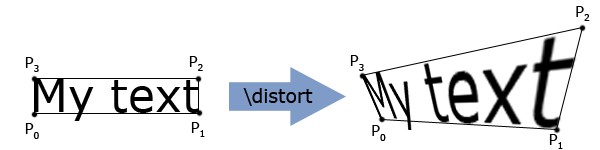
\includegraphics[width=0.7\textwidth]{./distort}
\end{center}

If the parameter list is ommitted, the distort reverts to the style's default (none by default).
This tag can be animated with \textbackslash t.

\textbf{Implementation:}
This tag cannot be reduced to an affine transformation, so it cannot be expressed in Matrix form.
In order to transform a given (x,y) coordinate pair to it:

\begin{enumerate}
\item Normalize the (x,y) coordinates to a (u,v) system, so that $P_0$ = (0,0) and $P_2$ = (1,1).
This can be done by dividing x by the block's baseline length (bl) and y by the block height (h).
The affine 3D transformation matrix for this operation is:\\
\begin{center}
$\displaystyle \begin{bmatrix}
\frac{1}{bl} & 0 & 0 & -\frac{P_{0x}}{bl} \\
0 & \frac{1}{h} & 0 & -\frac{P_{0y}}{h} \\
0 & 0 & 1 & 0 \\
0 & 0 & 0 & 1
\end{bmatrix}$
\end{center}
%\vspace{10pt}
That is, $\displaystyle u = \frac{P_x - P_{0x}}{bl}; v = \frac{P_y - P_{0y}}{h}$.
\item Apply the following formula: $P = P_0 + (P_1-P_0) u + (P_3-P_0) v + (P_0+P_2-P_1-P_3) u v$.\\
This can be interpreted as simple vector operations, that is, apply that once using the x coordinates
and another using the y coordinates. Since the four points are constant, the coeficients can be
precalculated, resulting in a very fast transformation.\\
\end{enumerate}

\subsubsection{\textbackslash baseline}

\textbf{Usage:}
\begin{verbatim}
\baseline(path1[,path2])
\end{verbatim}

\textbf{Description:}
Similarly to \textbackslash distort, this tag distorts the text, however, it does so by curving the
baseline into a vector path, so you can write curved text. Alternatively, you can specify a second
path to work as the ``ceiling'' of the text. The format of both path parameters is the standard
vector path format (see above).

\textbf{Implementation:}
Implementation of this tag can be summarized by the conversion of a generic $P_n = (x,y)$ point into
$P'_n = (x',y')$. Let $c1(t)$ and $c2(t)$ be the parametric equations of the two paths specified.
The conversion can then be done in the following manner:

\begin{enumerate}
\item Find the parameter \emph{t} along the baseline path that corresponds to the x position of
the point being converted. This can be done with a function that calculates the length from the
beginning of the path until an arbitrary point $P_t = c1(t)$ along it.
\item Calculate the base point along path1: $P_0 = c1(t)$
\item Calculate \emph{u} so that $u = \frac{y-y_0}{h}$, where $y_0$ is the y coordinate of the original
baseline and \emph{h} is the height of the block box.
\end{enumerate}

Now, for the single curve version:

\begin{enumerate}
\item Find the tangent vector of path1 at point $c1(t)$ and find the \emph{V} unit vector that is
perpendicular to the curve at that point, by rotating the tangent vector by -90 degrees along the Z axis.
This should give you a vector pointing ``up'', towards where the letters go. This can be summarized as:\\
$\displaystyle V = ( \lim_{h \to 0} (c1_y(t)-c1_y(t+h)) , \lim _{h\to0} (c1_x(t)-c1_x(t+h)))\\
V = \frac{V}{\left \| V \right \|}\\$
\todo Is that correct?
\item Multiply \emph{u} by the vector to find the offset from $P_0$, that is, $P'_n = P_0 + u V$.
\end{enumerate}

And for the two-curve version:

\begin{enumerate}
\item Calculate the ceiling point along path2: $P_1 = c2(t)$
\item Get \emph{P} with the parametric equation of the line defined by $(P_0,P_1)$: $P = (1-u) P_0 + u P_1$.
\end{enumerate}

\subsubsection{\textbackslash blpos}
\textbf{Usage:}
\begin{verbatim}
\blpos#
\end{verbatim}

\textbf{Description:}
This sets the position of the text relative to the baseline start. This tag can be animated.
\todo{Write proper specs for this.}

\subsection{Rastering Tags}
These tags affect how the subtitles are rasterized, that is, they affect things such as
colour, blurring, etc.

\subsubsection{\textbackslash \$vc}
\textbf{Usage:}
\begin{verbatim}
\$vc(colour1,colour2,colour3,colour4)
\end{verbatim}

\textbf{Description:}
Sets the primary colour to blend with each of the four vertices of draw polygon.
The primary use for this is to make smooth gradients easily, which are often required
for proper blending with the background. Note that you can also set alpha using this tag.

\subsubsection{\textbackslash \$blend}
\textbf{Usage:}
\begin{verbatim}
\$blend(mode)
\end{verbatim}

\textbf{Description:}
Sets the blending mode for the colour specified. Acceptable values are "normal", "add" and "multiply".

\subsubsection{\textbackslash clip}
\textbf{Usage:}
\begin{verbatim}
\clip(x1,y1,x2,x2)
\end{verbatim}

\textbf{Description:}
Clips so only text inside the rectangle formed by x1,y1,x2,y2 will be drawn

\subsubsection{\textbackslash iclip}
\textbf{Usage:}
\begin{verbatim}
\iclip(x1,y1,x2,x2)
\end{verbatim}

\textbf{Description:}
The inverse of \textbackslash clip, i.e. clips so only text outside the rectangle formed
by x1,y1,x2,y2 will be drawn.

\subsubsection{\textbackslash \$blur}
\textbf{Usage:}
\begin{verbatim}
\$blur(???)
\end{verbatim}

\textbf{Description:}
Blurs stuff. Animatable.

\todo{Gaussian kernel or a number of applications of box blur?}

\subsection{Advanced Typography Tags}
These are more advanced tags, which might prove to be fairly complex to implement. They include
things such as ruby text support (also known as furigana, when used with Japanese Kanji.)

\todo{Write me}


\newpage
\section{Renderer Behaviour Specification}
\todo{Write this section}


\newpage
\section{Container Multiplexing Specification}

\subsection{Matroska}
Storage of AS5 files in Matroska files is similar to how similar formats are stored.\cite{mkv ssa}
The Codec ID used is \textsc{S\_TEXT/AS5}

First, the entire file is converted to UTF-8 (if it isn't already UTF-8). Then, all sections other
than \emph{[Events]} and \emph{[Resources]} are stored on the \emph{CodecPrivate} element. For the
\emph{[Resources]} section, each line is parsed and files are converted to Matroska file attachments.
\todo{Specify this more clearly.}

Finally, each line in the \emph{[Events]} section is read and stored each in a block. The \emph{start}
and \emph{end} fields are parsed (see the specifications on the section describing [Events]) and set
as the \emph{TimeStamp} and \emph{BlockDuration} elements. The line itself is then stored in the
following format:

\begin{verbatim}
Line: readOrder,style,userData,contents
\end{verbatim}

Where \emph{readOrder} is the number that the line had on the file. This is necessary so the file
can be demultiplexed back in its original order, since lines will be stored in chronological order
while inside the Matroska file. The remaining fields should just be copied from the original line.


\newpage
\addcontentsline{toc}{section}{References}
\begin{thebibliography}{1}

\bibitem{Aegisub} Rodrigo Braz Monteiro, Niels Martin Hansen, David Lamparter et al., Aegisub. Application, 2005-2007.\\
\url{http://www.aegisub.net/}

\bibitem{asa} David Lamparter, asa. Application, 2004-2007.\\
\url{http://asa.diac24.net/}

\bibitem{SSA} Kotus, Sub Station Alpha. Website, 1997-2003.\\
\url{http://web.archive.org/web/*/http://www.eswat.demon.co.uk/substation.html}

\bibitem{ASS} \#Anime-Fansubs, Advanced Sub Station Alpha.\\
\url{http://www.anime-fansubs.org}\\
\url{http://moodub.free.fr/video/ass-specs.doc}

\bibitem{VSFilter} Gabest, VSFilter. Application, 2003-2007.\\
\url{http://sourceforge.net/projects/guliverkli/}

\bibitem{ASS3} David Lamparter, Advanced Sub Station Alpha 3. Website, 2007.\\
\url{http://asa.diac24.net/ass3.pdf}

\bibitem{mkv} The Matroska project. Website.\\
\url{http://www.matroska.org/}

\bibitem{UTF-8} The Internet Society, RFC 3629, ``UTF-8, a transformation format of ISO 10646''. Website, 2003.\\
\url{http://tools.ietf.org/html/rfc3629}

\bibitem{UTF-16} The Internet Society, RFC 2781, ``UTF-16, an encoding of ISO 10646''. Website, 2000.\\
\url{http://tools.ietf.org/html/rfc2781}

\bibitem{Unicode BOM} Unicode, Inc, The Unicode Standard, Chapter 13. PDF, 1991-2000.\\
\url{http://www.unicode.org/unicode/uni2book/ch13.pdf}

\bibitem{mkv ssa} The Matroska project, specification for SSA/ASS subtitle formats. Website.\\
\url{http://www.matroska.org/technical/specs/subtitles/ssa.html}

\end{thebibliography}

\end{document}